%
% File acl2015.tex

\documentclass[11pt]{article}
\usepackage{acl2015}
\usepackage{times}
\usepackage{url}
\usepackage{dsfont}
\usepackage{latexsym}
\usepackage{graphicx}


\title{Document Classification by Inversion of \\Distributed Language Representations}

\author{Matt Taddy \\
  University of Chicago Booth School of Business \\
  {\tt taddy@chicagobooth.edu} \\}

\date{}

\begin{document}
\maketitle
\begin{abstract}
There have been many recent advances in the structure and measurement of {\it distributed} language models: those that map from words to a vector-space that is rich in information about word choice and composition.  This vector-space is the distributed language representation.    

Given the success of such approaches,  researchers have proposed
models and algorithms to adapt them for use in document classification; e.g., for predicting sentiment.  The goal of this note is to point out that any distributed  representation can be turned into a classifier through inversion via Bayes rule.  
The approach is simple and modular, in that it will work with any language representation whose training can be formulated as optimizing a probability model. In our application to 2 million sentences from Yelp reviews, we also find that it performs as well as or better than  complex purpose-built algorithms. \end{abstract}

\section{Introduction}

Distributed, or vector-space, language representations consist of a location
for every vocabulary {\it word} in $\mathds{R}^d$, where $d$ is the dimension
of the latent representation space.  These locations are learned to optimize (or approximately optimize) an objective function defined on the original text, such as
a likelihood for word occurences.

A popular example is the word2vec machinery of \newcite{mikolov_distributed_2013}.  This 
trains the distributed representation to be useful as an input layer for prediction of
words from their neighbors in a Skip-gram likelihood; that is, to maximize 
\begin{equation}
\prod_{k\neq t,~k=t-b}^{t+b} \log\mathrm{p}(w_k\mid w_t)
\end{equation}
summed across all words $w_t$, where $b$ is a window (possibly truncated by the end or beginning of the sentence) and the function $\mathrm{p}(w_k\mid w_t)$ is a neural network classifier that depends upon vector-space representations for $w_k$ and $w_t$.

\section{word2vec}
The skip-gram probabalistic language model is trained to, for window $b$, maximize for each word

This probability is calculated for all possible word pairs over a sentence (some defined short chunk of language).

In the word2vec formulation, each probability is represented as

$$
\mathrm{p}(w \mid w_I) = \prod_{j=1}^{L(w)-1} \sigma\left( \mathrm{ch}\left[\eta(w,j+1)\right] \mathbf{u}_{\eta(w,j)}^\top \mathbf{v}_{w_I} \right)
$$

where 
* $\eta(w,i)$ is the $i^{th}$ node in a binary huffman tree representation (path) for word $w$, 
* $\sigma(x) = 1/(1 + \exp[-x])$,
* and $\mathrm{ch}(\eta) \in \{-1,+1\}$ translates from left/right child to +/- one.

The binary huffman tree represents each word as a series of bits, so that the probability of word $w$ given word $w_I$ can be written as the product of probabilities that each bit is either on or off (represented above through the $\mathrm{ch}$ function).

Given a fitted representation, we can score any new sentence (and sum across them for documents) according to the model \textit{implied} by the training process.  This gives a document (log) probability under that representation.  This can be calculated for language representations trained on each of the corpora associated with some class labels.  When combined with priors for each class label and inversion via Bayes rule, the document probabilities provide class probabilities.

The doc2vec tool maps from documents to a vector space of fixed dimension, which can then be used as input to off-the-shelf machine learners.  The latter builds the sentiment/meaning into the model itself, and conditions upon this information during the training process.

Advantages of the inversion framework include:
* modularity: it works for any model of language that can (or its training can) be interpreted as a probabilistic model.
* transparency and replicability: a simple extension of any software for training distributed language models.
* performance


\section{Example: Yelp Reviews}

\begin{quote}
``the food is always good i would highly recommend this place''
\end{quote}



\begin{figure*}
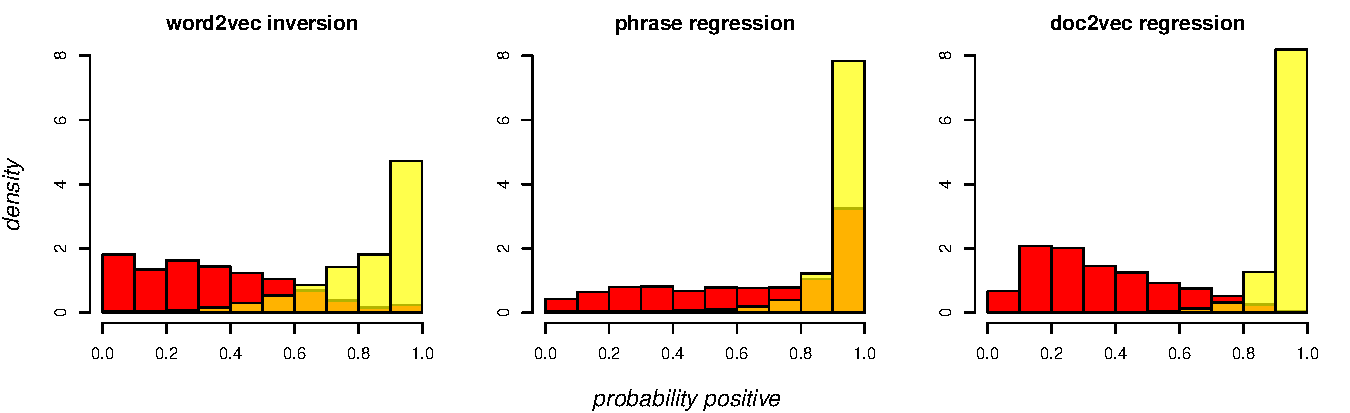
\includegraphics[width=\textwidth]{../graphs/coarseprob}

\vskip .5cm
\begin{center}
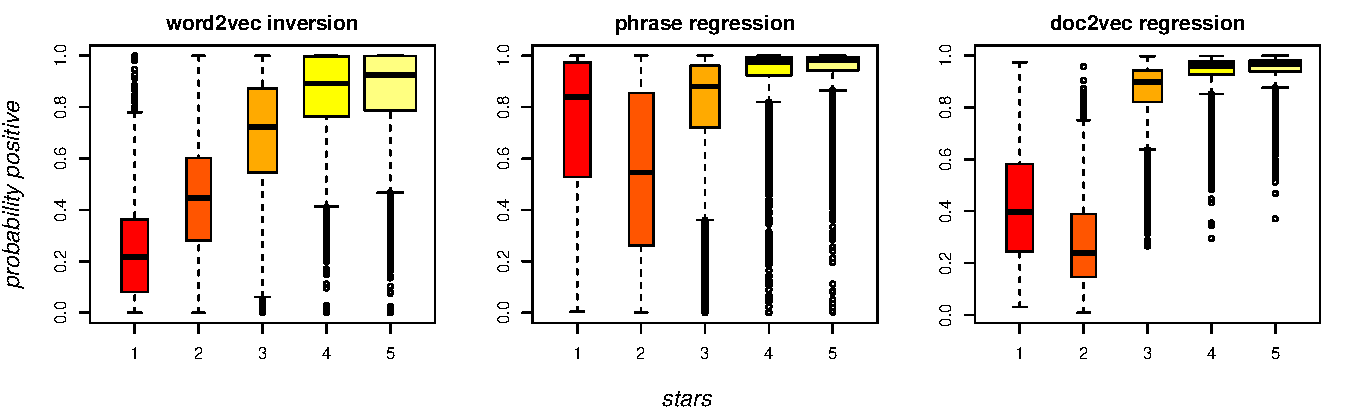
\includegraphics[width=.98\textwidth]{../graphs/coarseprob_bystar}
\end{center}
\vskip -.25cm
\caption{\label{pic:coarseprob} Out-of-Sample fitted probabilities of a review having greater than 2 stars. In the top histograms, red (dark) are the probabilities for true negative reviews and yellow (light) are for true positives.}
\end{figure*}
 


\begin{figure*}
\begin{center}
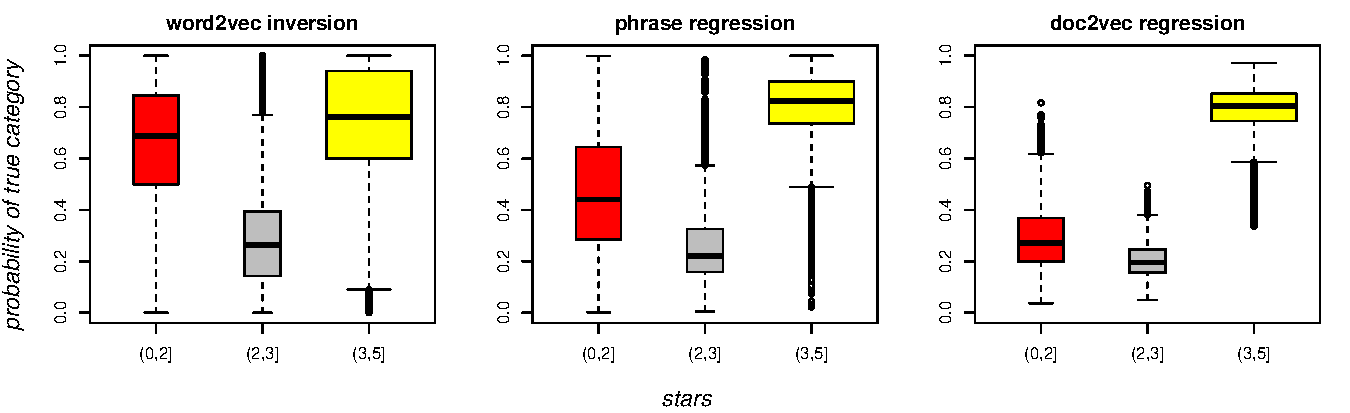
\includegraphics[width=.98\textwidth]{../graphs/nnpprob}

\vskip .25cm

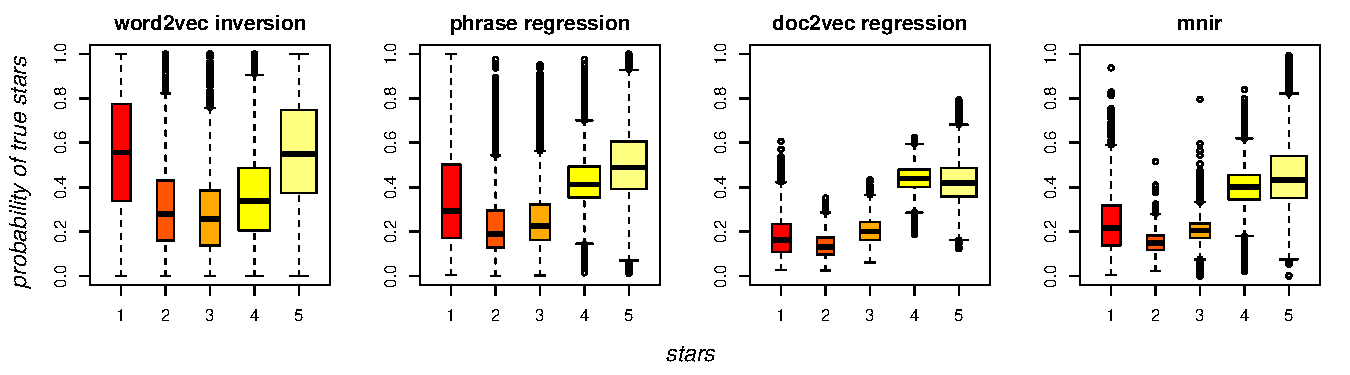
\includegraphics[width=.98\textwidth]{../graphs/fineprob}
\end{center}
\vskip -.25cm
\caption{\label{pic:fineprob} Out-of-Sample fitted probabilities for  observed truth.  In the top plot, we are predicting Negative ($\leq 2$), Neutral ($3$), or Positive ($\geq 4$).  In the bottom, we are predicting each of the separate 5 star ratings.}
\end{figure*}
 
\section{Discussion}

Engineering appeal: companies already fit w2v or some other distributed representation.  These could be done on a per-class basis instead, with prediction (e.g., of the next word) results averaged when the user class is unknown.  The current note makes it clear that such a system could act as the basis for document classification, as well as NLP\footnote{Training separate distributed representations for each class label has the separtate benefit of allowing computation to be partitioned across such labels, and thus fits with recent Big Data schemes such as EBF.}
\bibliographystyle{acl}
\bibliography{deepir}


\end{document}
